\documentclass[a4paper, 10pt, titlepage]{article}

\usepackage{inputenc,enumitem,graphicx,caption,float,amsmath,bbold,mathtools}
\usepackage[svgnames]{xcolor}
\usepackage[table]{xcolor}
\usepackage{listings}
\usepackage[left=2.5cm, right=4cm, top=2cm]{geometry}
\usepackage{makecell}
\usepackage[section]{placeins}
\makeatletter
\AtBeginDocument{%
  \expandafter\renewcommand\expandafter\subsection\expandafter{%
    \expandafter\@fb@secFB\subsection
  }%
}
\makeatother
\newcommand*\rot{\rotatebox{90}}
\newcommand\Tstrut{\rule{0pt}{2.9ex}}         % "top" strut
\newcommand\Bstrut{\rule[-1.2ex]{0pt}{0pt}}   % "bottom" strut
\newcommand\TBstrut{\Tstrut\Bstrut}           % "top and bottom" strut
\makeatletter
\def\verbatim{\small\@verbatim \frenchspacing\@vobeyspaces \@xverbatim}
\makeatother
\lstset{language=R,
    basicstyle=\small\ttfamily,
    stringstyle=\color{DarkGreen},
    otherkeywords={0,1,2,3,4,5,6,7,8,9},
    morekeywords={TRUE,FALSE},
    deletekeywords={data,frame,length,as,character},
    keywordstyle=\color{blue},
    commentstyle=\color{DarkGreen},
}

% \usepackage[english]{babel}
% \usepackage[utf8]{inputenc}
% \usepackage{amsmath,amsfonts}
% \usepackage{mathtools}
% \usepackage{graphicx}
% \usepackage{graphics}
% \usepackage[colorinlistoftodos]{todonotes}
% \usepackage[margin=1in]{geometry}
% \usepackage{enumitem}
% \usepackage{caption}
% \usepackage{multirow}
% \usepackage{fancyvrb}
% \usepackage{xcolor}
% \usepackage{float,bbold}
% \captionsetup[table]{skip=10pt}
% \newcommand*\rot{\rotatebox{90}}
% \usepackage[svgnames]{xcolor}
% \def\verbatim{\small\@verbatim \frenchspacing\@vobeyspaces \@xverbatim}
% \makeatother
% \lstset{language=R,
%     basicstyle=\small\ttfamily,
%     stringstyle=\color{DarkGreen},
%     otherkeywords={0,1,2,3,4,5,6,7,8,9},
%     morekeywords={TRUE,FALSE},
%     deletekeywords={data,frame,length,as,character},
%     keywordstyle=\color{blue},
%     commentstyle=\color{DarkGreen},
% }

\title{New Automobile Pricing}

\author{Submitted for January 2020 QEM by examinee 3159}

\date{January 5, 2020}

\begin{document}
\maketitle
\tableofcontents
\listoffigures
\listoftables

\newpage

\section*{Summary}
This study was initiated for the purpose of preparing a foreign automobile manufacturing company to enter the US market. The company's primary goal was to understand the factors governing the pricing of cars in the US, and to derive a model by which prices might be predicted from these factors. To this end, they obtained a data-set consisting of 215 observations of 26 variables concerning car manufacturing, technical specifications, and pricing, to which they provided our consulting firm. 
We begin by eliminating redundant variables and creating variables to categorize the brands of the vehicles in the data-set by their target market (economy, mid-range, or luxury). We also create a variable, log-price, which is the primary focus of our analysis throughout this report, and treat outliers in this variable by capping them at the 5$^{th}$ and 95$^{th}$ quantiles. 
After processing the data, we construct a LASSO regression model whose coefficients suggest that a manufacturer can expect to increase the price of a car by 0.25\% for each additional unit of width, increase the price by 0.02\% for each additional unit of curb weight, increase the price by 0.18\% for each additional unit of engine size, increase the price by 0.29\% for each additional horsepower, and decrease the price by around 24.17\% if targeting the economy market.

\section{Introduction}
A foreign automotive manufacturing corporation has is interested in expanding its operations to the US market. In preparation for this, the corporation has tasked our consulting firm with exploring the factors that determine the price of automobiles in the US. The primary objective of our study, then is to devise a model that might be used to predict the price of an automobile given its target market and manufacturing specifications.

\section{Data Summary}
The data consists of 215 observations of different automobiles currently sold in the US. The variables, listed in Table~\ref{table:orig data summary}, describe the brand and model, manufacturing specifications, and price of the automobiles in the data-set. Several adjustments were necessary before an analysis could be conducted. Firstly, we split the variable 'CarName' into two variables, one of which represented the brand of the car, and the other which represented the model. Although the data-set was known to contain 22 different brands, 5 observations referenced brands which were either abbreviated or spelled incorrectly; these were corrected and collapsed into the appropriate brand names. Splitting the data in this manner yielded complete pairings of brand and model for all but 2 observations, both of which had a missing model. Three other variables, `enginetype', `horsepower', and `enginelocation' also contained missing entries. In most cases, only one of the aforementioned variables contained a missing value; only one observation contained multiple missing entries. The full account of missing data is given in Table~\ref{table:missing data}. Observations with missing data in either `enginetype', `horsepower', or `enginelocation' were dropped from our initial analysis; we do, however, consider these observations later in our analysis.  

\begin{table}[!ht]
	\centering
	\captionof{table}{Summary of original car price data.}
	\begin{tabular}{|l|l|l|}
		\hline
		\textbf{Variable} & \textbf{Type} & \textbf{Levels}\\
		\hline
		Car\_ID & Integer & 215 IDs\\
		Symboling & Factor & -3, -2, -1, 0, 1, 2, 3\\
		CarName & Character & \\
		fueltype & Factor & gas, diesel\\
		aspiration & Factor & std, turbo\\
		doornumber & Factor & two, four\\
		carbody & Factor & \makecell[tl]{convertible, hatchback, \\sedan, wagon, hardtop\Bstrut}\\
		drivewheel & Factor & rwd, fwd, 4wd\\
		enginelocation & Factor & front, rear\\
		wheelbase & Continuous & \\
		carlength & Continuous & \\
		carwidth & Continuous & \\
		carheight & Continuous & \\
		curbweight & Continuous & \\
		enginetype & Factor & \makecell[tl]{dohc, ohcv, ohc, \\rotor, l, ohcf\Bstrut}\\
		cylindernumber & Factor & \makecell[tl]{four, six, five, three, \\twelve, two, eight\Bstrut}\\
		enginesize & Continuous & \\
		fuelsystem & Factor & \makecell[tl]{mpfi, 2bbl, mfi, 1bbl, \\spfi, 4bbl, idi, spdi\Bstrut}\\
		boreratio & Continuous & \\
		stroke & Continuous & \\
		compressionratio & Continuous & \\
		horsepower & Continuous & \\
		peakrpm & Continuous & \\
		citympg & Continuous & \\
		highwaympg & Continuous & \\
		price & Continuous & \\
		\hline
		\multicolumn{3}{|c|}{215 observations}\\
		\hline
	\end{tabular}
	\label{table:orig data summary}
\end{table}

\begin{table}[!ht]
	\centering
	\captionof{table}{Summary of missing data.}
	\begin{tabular}{|l|l|l|}
		\hline
		\textbf{Variable} & \textbf{\# Missing} & \textbf{\% Missing}\\
		\hline
		model & 2 & 0.1\%\\
		enginetype & 4 & 1.9\%\\
		horsepower & 10 & 4.7\%\\
		enginelocation & 41 & 19.1\%\\
		\hline
		\multicolumn{3}{|c|}{56 observations (26\% of data)}\\
		\hline
	\end{tabular}
	\label{table:missing data}
\end{table}

After removing the data containing missing values, we added two variables, `log\_price', the natural log of `price', and `bin', which indicates whether the car's brand caters to economy, mid-range, or luxury markets. We detail the determination of the `bin' later in our analysis. We also removed the variables `brand', which has been subsumed by bin, and `Car\_ID', which was found to be of little value. The transformed data-set is shown in Table~\ref{table:trans data summary}.

\begin{table}[!ht]
	\centering
	\captionof{table}{Summary of transformed car price data.}
	\begin{tabular}{|l|l|l|}
		\hline
		\textbf{Variable} & \textbf{Type} & \textbf{Levels}\\
		\hline
		Symboling & Ordinal & -3, -2, -1, 0, 1, 2, 3\\
		fueltype & Factor & gas, diesel\\
		aspiration & Factor & std, turbo\\
		doornumber & Factor & two, four\\
		carbody & Factor & \makecell[tl]{convertible, hatchback, \\sedan, wagon, hardtop\Bstrut}\\
		drivewheel & Factor & rwd, fwd, 4wd\\
		enginelocation & Factor & front, rear\\
		wheelbase & Continuous & \\
		carlength & Continuous & \\
		carwidth & Continuous & \\
		carheight & Continuous & \\
		curbweight & Continuous & \\
		enginetype & Factor & \makecell[tl]{dohc, ohcv, ohc, \\rotor, l, ohcf\Bstrut}\\
		cylindernumber & Factor & \makecell[tl]{four, six, five, three, \\twelve, two, eight\Bstrut}\\
		enginesize & Continuous & \\
		fuelsystem & Factor & \makecell[tl]{mpfi, 2bbl, mfi, 1bbl, \\spfi, 4bbl, idi, spdi\Bstrut}\\
		boreratio & Continuous & \\
		stroke & Continuous & \\
		compressionratio & Continuous & \\
		horsepower & Continuous & \\
		peakrpm & Continuous & \\
		citympg & Continuous & \\
		highwaympg & Continuous & \\
		price & Continuous & \\
		log\_price & Continuous & \\
		bin & Factor & econ, mid, lux\\
		\hline
		\multicolumn{3}{|c|}{159 observations}\\
		\hline
	\end{tabular}
	\label{table:trans data summary}
\end{table}

\section{Exploratory Data Analysis}
We begin our investigation by examining the variable of interest, price, through box-plots in Figure~\ref{figure:uncapped boxplot}.

\begin{figure}[!ht]
	\centering
	   \begin{tabular}{cc}
	      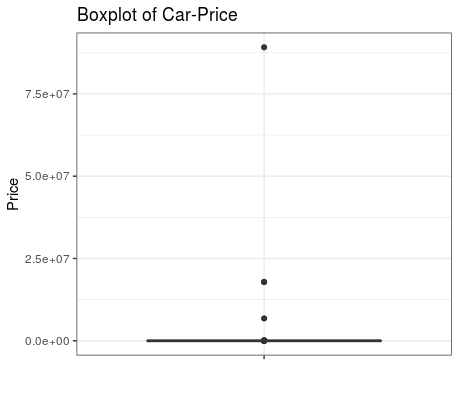
\includegraphics[width = 0.5\textwidth]{price.png}  & 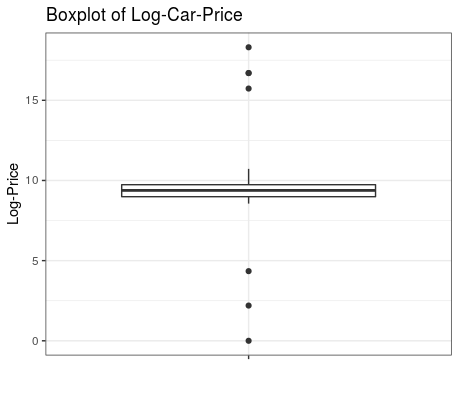
\includegraphics[width = 0.5\textwidth]{logprice.png} 
	   \end{tabular}
	\caption{Boxplots of price and log-price.}
	\label{figure:uncapped boxplot}
\end{figure}

Both the price and log-price distributions are severely distorted by outliers; capping the maximum and minimum values at the 5$^{th}$ and 95$^{th}$ quantile values of the log-price results in a more useful picture, which we can see in Figure~\ref{figure:capped density}.

\begin{figure}[!ht]
	\centering
	   \begin{tabular}{cc}
	      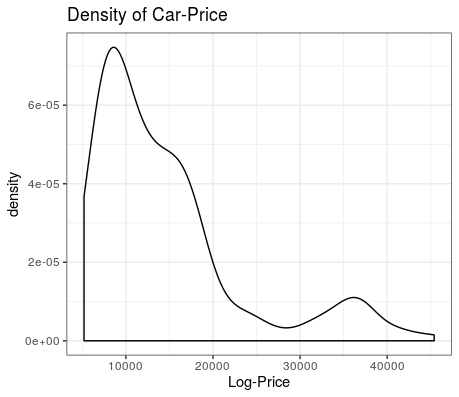
\includegraphics[width = 0.5\textwidth]{price_dense.png}  & 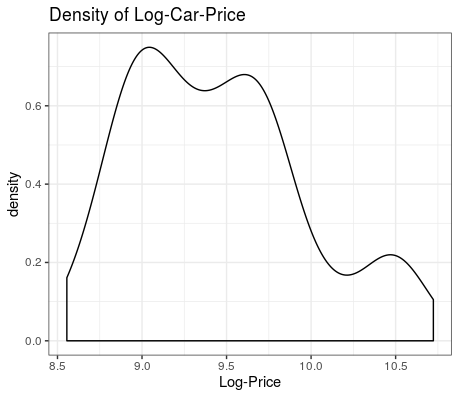
\includegraphics[width = 0.5\textwidth]{logprice_dense.png} 
	   \end{tabular}
	\caption{Density plots of price and log price after capping at 5$^{th}$ and 95$^{th}$ quantiles.}
	\label{figure:capped density}
\end{figure}

Notice the apparent trimodality of the capped log-price density; this may indicate that price is composed of several different distributions. For the remainder of this report, we consider the capped log-price and capped-price.

\par

We next investigate the possible response variables. We plot box-plots and scatter-plots of the relationship between the capped log-price and possible predictors in Figure~\ref{figure:resp box} and Figure~\ref{figure:resp scatter}.

	\begin{figure}[!ht]
	\centering
	    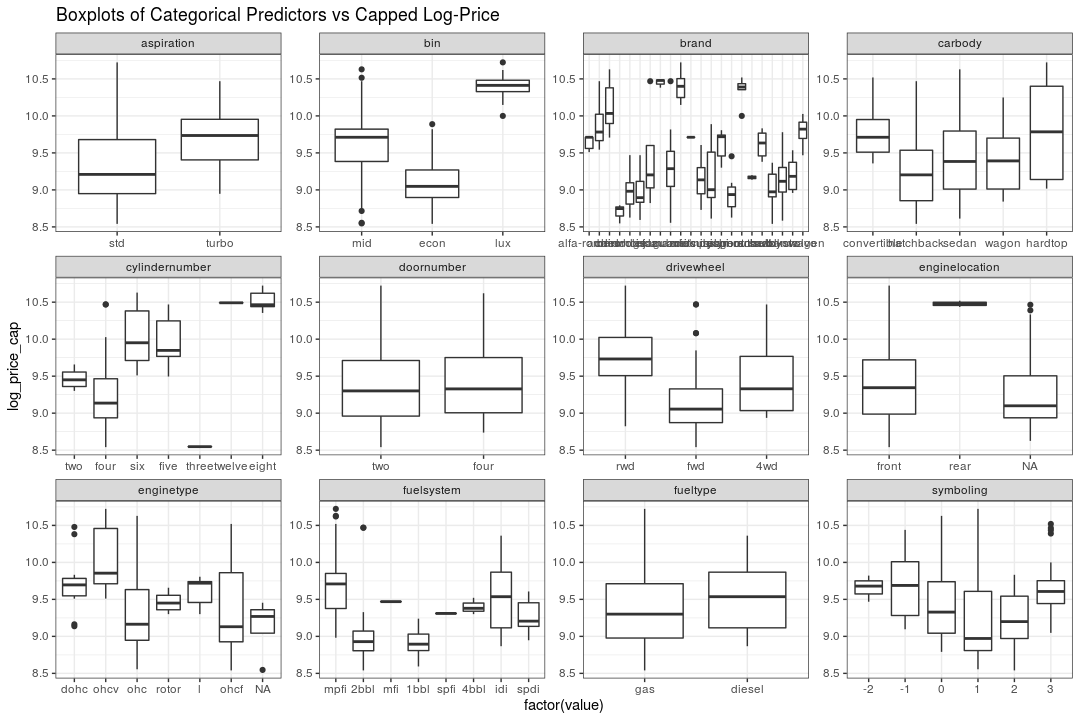
\includegraphics[width = 0.7\textwidth]{resp_box.png}
	\caption{Log-price vs categorical predictors.}
	\label{figure:resp box}
    \end{figure}

	\begin{figure}[!ht]
	\centering
	    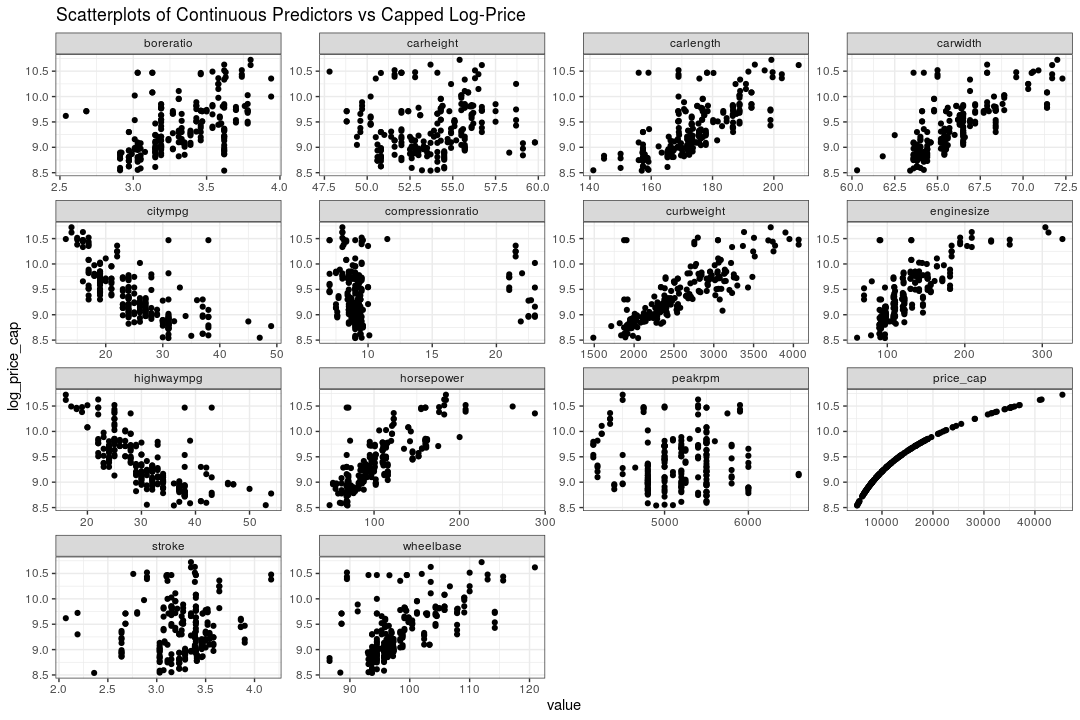
\includegraphics[width = 0.7\textwidth]{resp_scatter.png}
	\caption{Log-price vs continuous predictors.}
	\label{figure:resp scatter}
    \end{figure}
    
There appears to be a wide variation across the pricing tendencies of the various manufacturers, and among the continuous predictors, `carlength', `carwidth', `citympg', `curbweight', `enginesize', `highwaympg', and `horsepower' seem to show some evidence of a linear relationship with the capped log-price. However, upon plotting the correlation in Figure~\ref{figure:conts coll} between these predictor variables, we notice a high degree of collinearity, which indicates that much of the information about price explained by these variables is redundant.

	\begin{figure}[!ht]
	\centering
	    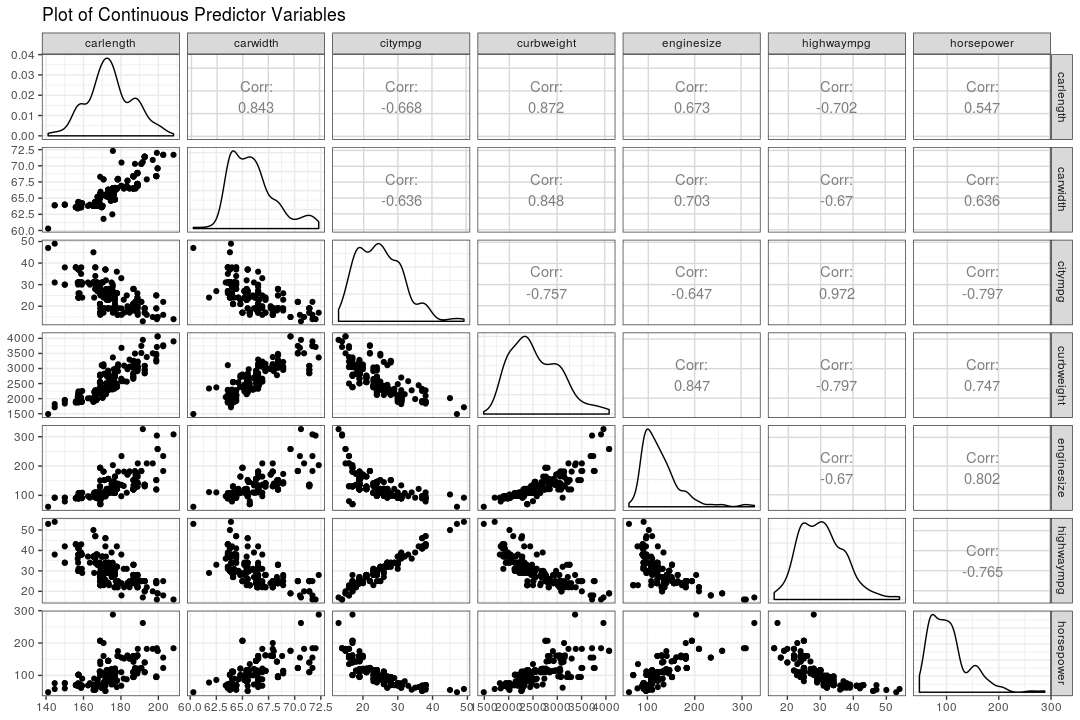
\includegraphics[width = 0.7\textwidth]{conts_var_pairs.png}
	\caption{Correlation between continuous variables.}
	\label{figure:conts coll}
    \end{figure}

\section{Analysis}
The trends that we have observed during our exploratory data analysis provide us with a framework under which to conduct our analysis.

\subsection{Binning Car Brands}
	We begin our statistical analysis by explaining the procedure by which we have binned the automobile brands into economy, mid-range, and luxury markets. As we saw in Figure~\ref{figure:capped density}, the distribution of the capped-log-price appears to be trimodal. In order to separate the three normal distributions the we suspect to comprise the capped-log-price, we apply the Expectation-Maximization algorithm. This algorithm allows us to detect latent variables that may influence a distribution, but not be represented in our data. The procedure operates by first assuming a distribution based on the data (in our case, we assume 3 different normal distributions), then calculating the probability that each data point within our sample of interest could be obtained from such a distribution. Based on these calculations, we assign the data to a class sharing this distribution. As we classify each data point, we then update our assumptions about the initial distributions.
	
	Applying the E-M algorithm to the distribution of log-price, we obtain the normal distributions pictured in Figure~\ref{figure:mixture dist}.
	
	\begin{figure}[!ht]
	\centering
	    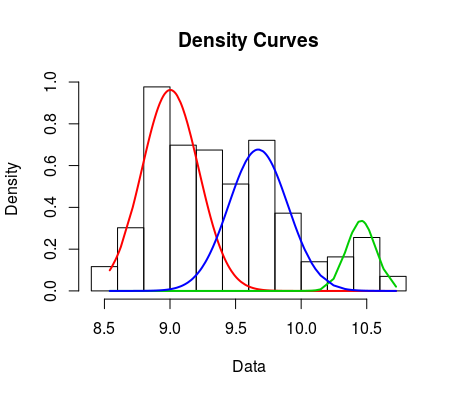
\includegraphics[width = 0.7\textwidth]{mixturedist.png}
	    \\
	    \begin{tabular}{lrr}
	         \textbf{Curve} & \textbf{$\mu$} & \textbf{$\sigma$} \\
	         \color{red}{Red} & 9.003 & 0.217\\
 	         \color{blue}{Blue} & 9.623 & 0.226\\
	         \color{green}{Green} & 10.457 & 0.112 \\
	    \end{tabular}
	\caption{Mixture distribution of capped-log-price.}
	\label{figure:mixture dist}
    \end{figure}
    
    Notice that there are three distributions with ascending mean values; we define the `economy' distribution to be the red curve, the `mid-range' distribution to be the blue curve, and the `luxury' distribution to be the green curve. After deriving the three Gaussian distributions, we calculated the mean log-price for each brand and placed the brand into the bin for whose density was highest at its mean log-price. The resulting bins are given in Table~\ref{table:bins}. A table of the calculated densities is given in the Appendix.
    
    \begin{table}[!ht]
	\centering
	\captionof{table}{Binned manufacturers.}
	\begin{tabular}{|l|l|}
		\hline
		\textbf{Bin} & \textbf{Manufacturers}\\
		\hline
		Economy & \makecell[tl]{Dodge, Honda, Mitsubishi, Nissan, Plymouth, Renault,\\ Subaru, Toyota, Volkswagen\Bstrut}\\
		Mid-range & \makecell[tl]{Alfa-Romero, Audi, BMW, Chevrolet, Isuzu, Mazda,\\ Mercury, Peugeot, Saab, Volvo\Bstrut}\\
		Luxury & Jaguar, Buick, Porsche\\
        \hline
	\end{tabular}
	\label{table:bins}
    \end{table}

\subsection{Price-Prediction Model}
We now address the issue of explaining the price of cars in the US market. We approach this problem by fitting a LASSO regression model to the data. The general LASSO model is given below.

\begin{align}
	\sum_{i=1}^{n} (y_i - \sum x_{ij}\beta_j)^2 + \lambda \sum_{j=1}^{p}\lvert \beta_j \rvert,
\end{align}

LASSO employs employs what is known as a shrinkage condition (governed in the above equation by $
lambda$) to fit a model for each $y_i$ (in our case, the log-capped-price). As the name suggests, this condition causes the coefficients (the $\beta_j$s in the above equation) of the explanatory variables (the $x_j$s in the equation) for the model to `shrink' toward 0. As $\lambda$ increases, the penalty becomes more severe, and more coefficients are eliminated. This has the desirable effect of producing a simple model, and is of particular utility when dealing with data for which multicollinearity is a concern. As we have seen in Figure~\ref{figure:conts coll}, there are several explanatory variables that exhibit signs of multicollinearity. 

To  perform our LASSO regression, we take 70\% of the data as a training set and reserve the remaining 30\% as a validation set. We then perform 10-fold cross-validation on our training set to obtain the $\lambda$ that minimizes the mean-squared-error of prediction. In our case, we take $\lambda =  0.0867$, and fitting to our test data set yields an MSE of 0.0557. The procedure for this cross-validation is given in the Appendix.

After fitting the LASSO model, we obtain the following coefficients:

    \begin{table}[!ht]
	\centering
	\captionof{table}{Coefficients from LASSO regression. Note that the model assumes a baseline bin of mid-range.}
	\begin{tabular}{|l|rr|}
		\hline
		\textbf{Variable} & \textbf{Coefficient} & \textbf{\makecell[r]{Exponentiated\\Coefficient}}\\
		\hline
		Intercept & 8.3537 & 4245.861\\
		Car Width & 0.0024 & 1.0025\\
		Curb Weight & 0.0002 & 1.0002\\
		Engine Size & 0.0018 & 1.0018\\
		Horsepower & 0.0029 & 1.0029\\
		Economy Bin & -0.2767 & 0.7583\\
        \hline
	\end{tabular}
	\label{table:coefs}
    \end{table}
    
Notice that many of the original explanatory variables are not present; as we have mentioned above, they have `shrunk' out of the model. 
    
Since our model fits log-price, our interpretation of the above is slightly more involved than multiplying the coefficient by the relevant explanatory variable. Instead, it is easiest to understand in terms of percentages; subtracting 1 from the exponentiated coefficient and multiplying by 100 tells us the expected percentage increase or decrease in price that comes from adding an additional unit to one of the explanatory variables, or by changing the category for factor variables. For example, we expect an 0.25\% increase in price for each additional unit of width added to the car, and we expect a 24.17\% decrease in price for economy vehicles. 

\section{Conclusion}
After analyzing the data, we arrive at the conclusion that the price of an automobile can accurately be predicted through car width, curb weight, engine size, horsepower, and market bin. A manufacturer can expect to increase the price of a car by 0.25\% for each additional unit of width, increase the price by 0.02\% for each additional unit of curb weight, increase the price by 0.18\% for each additional unit of engine size, increase the price by 0.29\% for each additional horsepower, and decrease the price by around 24.17\% if targeting the economy market.

\newpage

\section{Appendix}
\subsection{Additional Figures}

\begin{figure}[!ht]
	\centering
		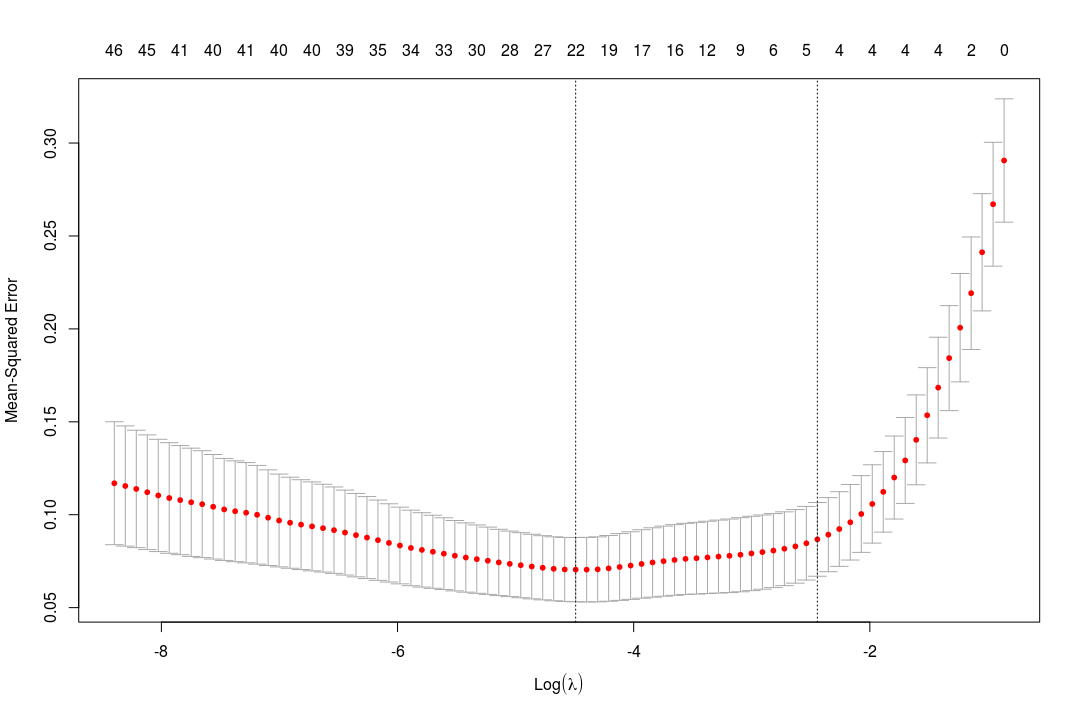
\includegraphics[width = 0.85\textwidth]{shrinkage.png}
	\caption{Plot of MSE by of shrinkage penalty.}
\end{figure}

\clearpage

\subsection{R Output}
\begin{lstlisting}[basicstyle = \footnotesize \ttfamily]
###BINNING MANUFACTURERS###
> #density at mean log price for economy, mid-range, or luxury dists
> print(
+ car_price_cap %>%
+   group_by(brand) %>%
+   summarize(mean_log_price = mean(log_price_cap)) %>%
+   mutate(p_econ = dnorm(mean_log_price, mix_lp$mu[1], mix_lp$sigma[1]),
+          p_mid = dnorm(mean_log_price, mix_lp$mu[3], mix_lp$sigma[3]),
+          p_lux = dnorm(mean_log_price, mix_lp$mu[2], mix_lp$sigma[2])), n = Inf)
# A tibble: 22 x 5
   brand       mean_log_price   p_econ    p_mid    p_lux
   <fct>                <dbl>    <dbl>    <dbl>    <dbl>
 1 alfa-romero           9.64 2.28e- 2 1.75     1.44e-11
 2 audi                  9.87 5.53e- 4 1.19     5.01e- 6
 3 bmw                  10.1  3.22e- 6 0.255    3.62e- 2
 4 chevrolet             8.70 6.73e- 1 0.000152 1.18e-53
 5 dodge                 9.00 1.84e+ 0 0.0213   1.09e-36
 6 honda                 8.98 1.84e+ 0 0.0167   1.29e-37
 7 isuzu                 9.42 2.76e- 1 0.964    1.47e-18
 8 jaguar               10.5  3.59e-10 0.00473  3.55e+ 0
 9 mazda                 9.31 6.91e- 1 0.472    5.17e-23
10 buick                10.4  1.36e- 9 0.00905  3.21e+ 0
11 mercury               9.71 8.68e- 3 1.74     9.19e-10
12 mitsubishi            9.14 1.51e+ 0 0.108    4.02e-30
13 nissan                9.17 1.35e+ 0 0.153    1.44e-28
14 peugeot               9.61 3.81e- 2 1.69     1.14e-12
15 plymouth              8.95 1.79e+ 0 0.0104   2.24e-39
16 porsche              10.3  9.62e- 9 0.0226   2.05e+ 0
17 renault               9.17 1.37e+ 0 0.146    8.75e-29
18 saab                  9.62 3.35e- 2 1.71     2.20e-12
19 subaru                9.03 1.83e+ 0 0.0301   2.34e-35
20 toyota                9.15 1.44e+ 0 0.126    1.90e-29
21 volkswagen            9.20 1.23e+ 0 0.193    1.64e-27
22 volvo                 9.79 2.66e- 3 1.56     6.02e- 8

###CROSS VALIDATION###
> preds <- tibble(actual = y_test, 
+                 fitted = predict(car_lasso, s = best_lamb, newx = x_test))
> print(preds, n = Inf)
# A tibble: 45 x 2
   actual fitted[,"1"]
    <dbl>        <dbl>
 1  10.1          9.81
 2   9.71         9.49
 3   9.74         9.49
 4   9.30         8.98
 5   8.98         9.14
 6   9.05         9.16
 7   9.10         9.27
 8  10.5         10.7 
 9   8.56         9.26
10   9.52         9.43
11   9.09         9.47
12   9.05         9.48
13   9.81         9.67
14  10.4         10.00
15   9.30         8.99
16   8.73         9.00
17   9.61         9.54
18   8.80         9.00
19   8.90         9.03
20   8.99         9.03
21   9.16         9.21
22   9.49         9.73
23   9.54         9.78
24   9.74         9.74
25   9.72         9.65
26   8.81         9.00
27   9.10         9.23
28  10.00         9.78
29   9.38         9.60
30   9.41         9.61
31   9.83         9.78
32   8.54         9.03
33   8.99         9.17
34   8.84         9.04
35   8.96         9.07
36   8.99         9.06
37   9.02         9.07
38   9.32         9.39
39   9.78         9.45
40   9.10         9.21
41   9.01         9.14
42   9.21         9.20
43   9.36         9.16
44   9.47         9.70
45   9.68         9.71
> MSPE <- mean((preds$actual - preds$fitted)^2)
> MSPE
[1] 0.05567646
\end{lstlisting}

\subsection{R Code}
\begin{lstlisting}[basicstyle = \footnotesize \ttfamily]
library(tidyverse)
library(broom)
library(ggplot2)
library(ggmosaic)
library(GGally)
library(stringdist)
library(modeest)
library(mixtools)
library(glmnet)

ggplot2::theme_set(ggplot2::theme_bw())

car_price_orig <- read_csv("CarPrice.csv") %>%
  separate(CarName, c("brand", "model"), sep = " ", extra = "merge", 
           fill = "right") %>%
  mutate(enginetype = ifelse(.$enginetype %in% c("dohc", "ohc", "ohcv",
                                                 "rotor", "l", "ohcf"), 
                             enginetype, NA))

#checking for missing values
colSums(is.na(car_price_orig))
215*(1-mean(complete.cases(car_price_orig))) #num of missing obs

#checking frequency of engine locations
count(car_price_orig, enginelocation)

#checking frequency of engine types
count(car_price_orig, enginetype)

#checking NAs
view(filter(car_price_orig, is.na(model)))
view(filter(car_price_orig, is.na(enginelocation)))
view(filter(car_price_orig, is.na(horsepower)))
view(filter(car_price_orig, is.na(enginetype)))

#vector of properly-spelled brand names
brands <- setdiff(car_price_orig$brand, 
                  c("porscshce", "toyouta", "volkw", "vokswagen"))

car_price_trans <- car_price_orig %>%
          #matching misspelled brand names to correctly-spelled names
  mutate(brand = brands[amatch(.$brand, brands, method = "jw", maxDist = 5)],
         #creating log-price variable
         log_price = log(price)) %>%
  #creating unordered factor variables
  mutate_at(c("symboling", "brand", "fueltype", "aspiration", "doornumber",
              "carbody", "drivewheel", "enginelocation", "enginetype", 
              "cylindernumber", "fuelsystem"), as_factor) %>%
  #dropping unused variables
  dplyr::select(-c("car_ID", "model"))

#capping price outliers at 5th and 95th %-tile
q <- 1.5*IQR(car_price_trans$log_price)
qnt <- quantile(car_price_trans$log_price, prob = c(0.25, 0.75))
caps <- quantile(car_price_trans$log_price, prob = c(0.5, 0.95))

car_price_cap <- car_price_trans %>% 
  mutate(log_price_cap = if_else(log_price < qnt[1] - q, caps[1],
                          if_else(log_price > qnt[2] + q, caps[2], log_price))) %>%
  mutate(price_cap = exp(log_price_cap)) %>%
  dplyr::select(-c(price, log_price))

 #######
## EDA ##
 #######

#boxplot of price
car_price_trans %>%
  ggplot(aes(x = "", y = price)) +
  geom_boxplot() +
  ylab("Price") +
  xlab("") +
  ggtitle("Boxplot of Car-Price")

car_price_trans %>%
  ggplot(aes(x = "", y = log_price)) +
  geom_boxplot() +
  ylab("Log-Price") +
  xlab("") +
  ggtitle("Boxplot of Log-Car-Price")

#boxplot of capped log-price
car_price_cap %>%
  ggplot(aes(x = "", y = price_cap)) +
  geom_boxplot() +
  ylab("Price") +
  xlab("") +
  ggtitle("Boxplot of Car-Price")

car_price_cap %>%
  ggplot(aes(x = "", y = log_price_cap)) +
  geom_boxplot() +
  ylab("Log-Price") +
  xlab("") +
  ggtitle("Boxplot of Log-Car-Price")

#density plot of capped price
car_price_cap %>%
  ggplot(aes(x = price_cap)) +
  geom_density() +
  xlab("Log-Price") +
  ggtitle("Density of Car-Price")

car_price_cap %>%
  ggplot(aes(x = log_price_cap)) +
  geom_density() +
  xlab("Log-Price") +
  ggtitle("Density of Log-Car-Price")

#mixture distribution of log-price
mix_lp <- normalmixEM(car_price_cap$log_price_cap, k = 3)
mix_lp

mix_lp$mu[2]

#plot of mixture distribution
plot(mix_lp, which = 2)

#density at mean log price for economy, mid-range, or luxury dists
car_price_cap %>%
  group_by(brand) %>%
  summarize(mean_log_price = mean(log_price_cap)) %>%
  mutate(p_econ = dnorm(mean_log_price, mix_lp$mu[1], mix_lp$sigma[1]),
         p_mid = dnorm(mean_log_price, mix_lp$mu[3], mix_lp$sigma[3]),
         p_lux = dnorm(mean_log_price, mix_lp$mu[2], mix_lp$sigma[2])) %>%
  view

car_price_binned <- car_price_cap %>%
         #creating bins for economy, luxury, mid-range cars
  mutate(bin = as_factor(if_else(brand %in% c("alfa-romero", "audi", "bmw", 
                                    "chevrolet", "isuzu", "mazda", 
                                    "mercury", "peugeot", "saab", 
                                    "volvo"),
                       "mid",
                if_else(brand %in% c("jaguar", "buick", "porsche"),
                        "lux", "econ")))) %>%
  #dropping brand
  dplyr::select(-brand)

View(count(car_price_binned, bin, brand))

#scatterplots of log-price against conts vars
car_price_binned %>%
  select_if(is.numeric) %>%
  pivot_longer(-log_price_cap, names_to = "var", values_to = "value") %>%
  ggplot(aes(x = value, y = log_price_cap)) +
  geom_point() +
  facet_wrap(~var, scales = "free") +
  ggtitle("Scatterplots of Continuous Predictors vs Capped Log-Price")

#boxplots of log-price against categorical vars
non_numeric <- !sapply(car_price_binned, is.numeric)
car_price_binned %>%
  dplyr::select("log_price_cap", names(non_numeric)[as.numeric(non_numeric) == 1]) %>%
  pivot_longer(-log_price_cap, names_to = "var", values_to = "value") %>%
  ggplot(aes(x = factor(value), y = log_price_cap)) +
  geom_boxplot() +
  facet_wrap(~var, scales = "free") +
  ggtitle("Boxplots of Categorical Predictors vs Capped Log-Price")

#scatterplots of continuous predictors against each other
car_price_binned %>%
  select(carlength, carwidth, citympg, curbweight, enginesize,
         highwaympg, horsepower) %>%
  ggpairs(title = "Plot of Continuous Predictor Variables")

 ##########
# Analysis #
 ##########

#splitting into training and testing
car_price_nona <- car_price_binned %>%
  drop_na

train <- car_price_nona %>%
  sample_frac(0.7)
test <- car_price_nona %>%
  setdiff(train)

x_train = model.matrix(log_price_cap~.+I(enginesize^2)-1-price_cap, train)[,-1]
x_test = model.matrix(log_price_cap~.+I(enginesize^2)-1-price_cap, test)[,-1]

y_train = train %>%
  select(log_price_cap) %>%
  unlist() %>%
  as.numeric()

y_test = test %>%
  select(log_price_cap) %>%
  unlist() %>%
  as.numeric()

#choosing best lambda by 10-fold cross-validation
set.seed(2020)

car_lasso <- cv.glmnet(x_train, y_train)
best_lamb <- car_lasso$lambda.1se
best_lamb
coef(car_lasso)
plot(car_lasso)

preds <- tibble(actual = y_test, 
                fitted = predict(car_lasso, s = best_lamb, newx = x_test))
MSPE <- mean((preds$actual - preds$fitted)^2)
MSPE
\end{lstlisting}

\end{document}

